%=======================================================
\section{Monitoring mit Skripten}
%=======================================================
Für die Überwachung von speziellen Anwendungen oder Arbeitsabläufen, reichen bestehende standardisierte Managementagenten häufig nicht aus. Die notwendigen Statusinformationen können über Standard- oder Herstellerspezifische \emph{SNMP\footnote{SNMP ist das Simple Network Management Protocol} MIB}\footnote{Management Information Base} nicht abgefragt werden. Um hier spezielle Anforderungen erfüllen zu können ist es möglich eigene Programme oder Skripte zur Überwachung einzubinden. Um ein möglichst praxisnahes und durchgängiges Beispiel liefern zu können, konfigurieren wir exemplarisch eine Festplattenüberwachung mit \emph{S.M.A.R.T}\footnote{Self-Monitoring, Analysis and Reporting Technology}. Um die Abläufe zu verdeutlichen richten wir einen  Monitor ein, der den Zustand einer lokal installieren Festplatte überwacht.

Die Verwendung der eigenen Programme und Skripte kann auf unterschiedliche Art und Weise realisiert werden. Im ersten Teil wird beschrieben, wie der unter \emph{Unix/Linux} weit verbreitete \emph{Net-SNMP} Agent erweitert und in \emph{OpenNMS} genutzt werden kann. Das Monitoring des Festplattenstatus wird in Varianten durchgeführt und soll den Ablauf und die Notwendigen Konfigurationsschritte verdeutlichen.

\emph{Nagios}, als ein weit verbreitetes quelloffenes Monitoringsystem, stellt einen sehr großen Pool\footnote{Nagios Plugins unter \url{http://www.monitoringexchange.org}} von Überwachungsskripten und Programmen zur Verfügung. Diese Skripte können als \emph{Plugins} auf einem Server mit einem \emph{Nagios-Agenten}\footnote{Unter Linux/Unix \emph{NRPE} unter Windows \emph{NSClient++}} ausgeführt werden. In diesem Dokument wird beschrieben wie \emph{OpenNMS} die \emph{NRPE} Agenten in der Netzwerküberwachung nutzen kann. In \emph{OpenNMS} wird dazu ein spezieller \emph{NRPE Monitor} bereitgestellt. Er veranlasst das ausführen der \emph{Plugins} und stellt den Status entsprechend dar.

Da für die Verwaltung von \emph{Unix/Linux} basierten Systemen häufig das SSH-Protokoll\footnote{Secure Shell} verwendet wird, kann auch dieses Protokoll für die Netzwerküberwachung verwendet werden. Es erlaubt neben der Bereitstellung eines entfernten Shellzugangs ebenfalls die Möglichkeit, Programme oder Skripte auf dem entfernten Server auszuführen. In \emph{OpenNMS} kann dazu der \emph{General Purpose Monitor} verwendet werden. Er erlaubt es Shellkommandos auszuführen und kann das Ergebnis des Kommandos in einem \emph{Service Status} auswerten.

Das \emph{HTTP\footnote{Hyper Text Transfer Protokoll}} ist eines der wichtigsten Protokolle im Internet. Es wird neben der Auslieferung von Internetseiten auch für entfernte Funktionsaufrufe (\emph{ReST\footnote{Representational State Transfer}} oder \emph{SOAP}\footnote{Simple Object Access Protocol}) genutzt. Zusätzlich lässt sich \emph{HTTP} auch für Monitoring-Zwecke verwenden. Über \emph{HTTP} können sowohl Statusabfragen oder auch Leistungsdaten für das Monitoring bereitgestellt werden. Die Übertragung kann zudem über \emph{SSL\footnote{Secure Socket Layer}} verschlüsselt erfolgen. Zusätzlich sind Webserver nahezu auf jedem System sehr einfach einzurichten und sind im Netzwerk oft gut erreichbar. Im letzten Abschnitt wird gezeigt wie man einen \emph{Apache2-Server\footnote{Apache Project: \url{http://httpd.apache.org}}} in Verbindung mit \emph{CGI\footnote{Common Gateway Interface}} für das Monitoring in \emph{OpenNMS} einrichten kann. Der Fokus liegt hier auf dem Statusmonitoring. Auf eine \emph{HTTP-Datacollection\footnote{OpenNMS HTTP-Datacollection im OpenNMS Wiki}} zur Aufzeichnung von Leistungsdaten wird hier nicht eingegangen.

%=======================================================
\subsection{Einrichtung von S.M.A.R.T.}
%=======================================================
Um die Beispiele einrichten und nachvollziehen zu können muss voerst sicher gestellt werden, dass die \emph{S.M.A.R.T.-Tools} installiert und eingerichtet sind. Das folgende Beispiel wurde auf einem \emph{Ubuntu 9.10 Server} durchgeführt. Die \emph{S.M.A.R.T.-Tools} können mit dem folgenden Kommando installiert werden.

\begin{lstlisting}[numbers=none]
aptitude install smartmontools
\end{lstlisting}

Für die Plattenüberwachung muss zusätzlich noch ein Prozess gestartet werden, der die entsprechenden Informationen von den Festplatten ausliest.

\begin{lstlisting}[numbers=none]
vi /etc/default/smartmontools
\end{lstlisting}

Zunächst muss erlaubt werden, dass der \emph{smartd} gestartet werden kann und welche Festplatten überwacht werden sollen. In unserem Beispiel werden die beiden Festplatten \emph{/dev/sda} und \emph{/dev/sdb} überwacht. Die Konfigurationsdatei sieht dann wie folgt aus:

\lstinputlisting[caption={Konfiguration der \emph{smartmontools}}
      \label{lst:smartmontools-config}]
  {configs/use-cases/script-extending-linux/smartmontools}

Der Dienst kann anschließend mit dem Kommando

\begin{lstlisting}[numbers=none]
service smartmontools start
\end{lstlisting}

gestartet werden. Um zu testen ob die Festplatteninformationen korrekt ausgelesen werden, kann das folgende Kommando den aktuellen Status liefern.

\begin{lstlisting}[numbers=none]
smartctl -H /dev/sdb
\end{lstlisting}

\lstinputlisting[caption={Ausgabe von \emph{smartctl}}
      \label{lst:smartctl-output}]
  {configs/use-cases/script-extending-linux/smartctl-output.txt}

Wenn die folgende Ausgabe wie oben gezeigt aussieht, dann können wir mit dem Einrichten der Überwachung fortfahren.

In den nächsten Abschnitten wird ein Monitoring mit den eben installierten smartmontools beschrieben. Wir beginnen zunächst mit der Variante über \emph{Net-SNMP}. Im Anschluss wird das gleiche Monitoring über \emph{NRPE}, über \emph{SSH} und auch über \emph{HTTP} mittels \emph{CGI} dargestellt.

\subsection{Net-SNMP als Agenten}
In \emph{Unix/Linux} Umgebungen kommt häufig \emph{Net-SNMP} als Agent zum Einsatz. Dieser stellt damit nicht nur den Zugriff für die in der \emph{Standard MIB-II} definierten Managementobjekte bereit, sondern erlaubt es zusätzlich eigene Skripte per \emph{SNMP} einzubinden. Diese Möglichkeit macht damit die Skripte und Programme nicht nur für \emph{OpenNMS} zugänglich, sondern können auch in jeder anderen \emph{SNMP-fähigen} Netzwerküberwachungsanwendung verwendet werden. In diesem Beispiel wird gezeigt wie ein Shellskript in \emph{Net-SNMP} eingebunden wird. Die Ausgabe des Skriptes wird mit dem \emph{OpenNMS} bereitgestellten \emph{SNMP-Monitor} überwacht und als \emph{Service-Status} dargestellt. In der folgenden Abbildung wird der Ablauf grob skizziert.

\begin{figure}[H]
	\centering
	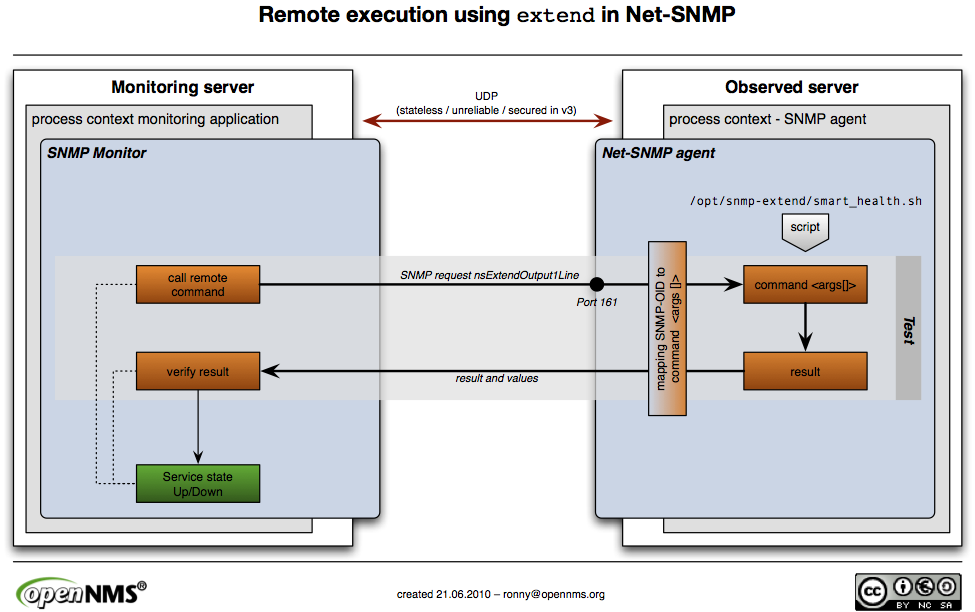
\includegraphics[width=1.0\textwidth]{images/use-cases/script-extending-linux/flow-netsnmp}
	\caption{Ablauf von Abfragen mit der Erweiterung des \emph{Net-SNMP} Agenten}
	\label{pic:flow-netsnmp}
\end{figure}
